\documentclass[usenames,dvipsnames,tikz]{standalone}
\usepackage{xcolor}
\colorlet{myBlue}{RoyalBlue!35!Cerulean}
\colorlet{myRed}{Red}
\usepackage{tikz}
\usepackage{standalone}
\begin{document}	
	
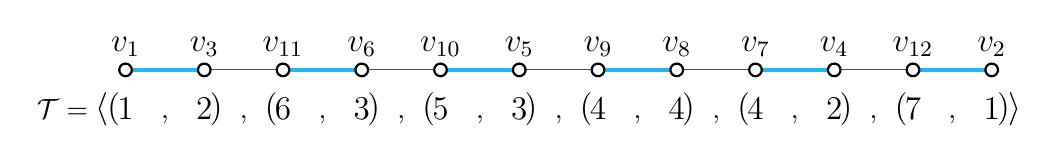
\begin{tikzpicture}
%\draw [help lines] (-1,-1) grid (14, 6);

\draw [ultra thick, myBlue] (1,3) -- (2,3);
\draw [ultra thick, myBlue] (3,3) -- (4,3);
\draw [ultra thick, myBlue] (5,3) -- (6,3);
\draw [ultra thick, myBlue] (7,3) -- (8,3);
\draw [ultra thick, myBlue] (9,3) -- (10,3);
\draw [ultra thick, myBlue] (11,3) -- (12,3);

\draw [myRed] (2,3) -- (3,3);
\draw [myRed] (4,3) -- (5,3);
\draw [myRed] (6,3) -- (7,3);
\draw [myRed] (8,3) -- (9,3);
\draw [myRed] (10,3) -- (11,3);

\draw [fill=white, thick] (1,3) circle [radius = 0.08];
\draw [fill=white, thick] (2,3) circle [radius = 0.08];
\draw [fill=white, thick] (3,3) circle [radius = 0.08];
\draw [fill=white, thick] (4,3) circle [radius = 0.08];
\draw [fill=white, thick] (5,3) circle [radius = 0.08];
\draw [fill=white, thick] (6,3) circle [radius = 0.08];
\draw [fill=white, thick] (7,3) circle [radius = 0.08];
\draw [fill=white, thick] (8,3) circle [radius = 0.08];
\draw [fill=white, thick] (9,3) circle [radius = 0.08];
\draw [fill=white, thick] (10,3) circle [radius = 0.08];
\draw [fill=white, thick] (11,3) circle [radius = 0.08];
\draw [fill=white, thick] (12,3) circle [radius = 0.08];

\node [above] at (1,3.05) {\large{$v_1$}};
\node [above] at (2,3.05) {\large{$v_3$}};
\node [above] at (3,3.05) {\large{$v_{11}$}};
\node [above] at (4,3.05) {\large{$v_6$}};
\node [above] at (5,3.05) {\large{$v_{10}$}};
\node [above] at (6,3.05) {\large{$v_5$}};
\node [above] at (7,3.05) {\large{$v_9$}};
\node [above] at (8,3.05) {\large{$v_8$}};
\node [above] at (9,3.05) {\large{$v_7$}};
\node [above] at (10,3.05) {\large{$v_4$}};
\node [above] at (11,3.05) {\large{$v_{12}$}};
\node [above] at (12,3.05) {\large{$v_2$}};

\node at (1,2.5) {\large{1}};
\node at (2,2.5) {\large{2}};
\node at (3,2.5) {\large{6}};
\node at (4,2.5) {\large{3}};
\node at (5,2.5) {\large{5}};
\node at (6,2.5) {\large{3}};
\node at (7,2.5) {\large{4}};
\node at (8,2.5) {\large{4}};
\node at (9,2.5) {\large{4}};
\node at (10,2.5) {\large{2}};
\node at (11,2.5) {\large{7}};
\node at (12,2.5) {\large{1}};

\node at (1.5,2.37) {,};
\node at (2.5,2.37) {,};
\node at (3.5,2.37) {,};
\node at (4.5,2.37) {,};
\node at (5.5,2.37) {,};
\node at (6.5,2.37) {,};
\node at (7.5,2.37) {,};
\node at (8.5,2.37) {,};
\node at (9.5,2.37) {,};
\node at (10.5,2.37) {,};
\node at (11.5,2.37) {,};

\node at (0.85,2.5) {\large{(}};
\node at (2.15,2.5) {\large{)}};
\node at (2.85,2.5) {\large{(}};
\node at (4.15,2.5) {\large{)}};
\node at (4.85,2.5) {\large{(}};
\node at (6.15,2.5) {\large{)}};
\node at (6.85,2.5) {\large{(}};
\node at (8.15,2.5) {\large{)}};
\node at (8.85,2.5) {\large{(}};
\node at (10.15,2.5) {\large{)}};
\node at (10.85,2.5) {\large{(}};
\node at (12.15,2.5) {\large{)}};

\node at (0.7, 2.5) {\large{$\langle$}};
\node at (12.3, 2.5) {\large{$\rangle$}};

\node at (0.2, 2.5) {$\mathcal{T} =$};


%\node [below] at (1,3) {1};
%\node [below] at (2,3) {2};
%\node [below] at (3,3) {6};
%\node [below] at (4,3) {3};
%\node [below] at (5,3) {5};
%\node [below] at (6,3) {3};
%\node [below] at (7,3) {4};
%\node [below] at (8,3) {4};
%\node [below] at (9,3) {4};
%\node [below] at (10,3) {2};
%\node [below] at (11,3) {7};
%\node [below] at (12,3) {1};

%\node [above] at (1,3) {$v_1$};
%\node [above] at (2,3) {$v_3$};
%\node [above] at (3,3) {$v_{11}$};
%\node [above] at (4,3) {$v_6$};
%\node [above] at (5,3) {$v_{10}$};
%\node [above] at (6,3) {$v_5$};
%\node [above] at (7,3) {$v_9$};
%\node [above] at (8,3) {$v_8$};
%\node [above] at (9,3) {$v_7$};
%\node [above] at (10,3) {$v_4$};
%\node [above] at (11,3) {$v_{12}$};
%\node [above] at (12,3) {$v_2$};










\end{tikzpicture}
	
\end{document}
